\documentclass[11pt,a4paper]{article}
\usepackage[margin=1in]{geometry}
\usepackage[T1]{fontenc}
\usepackage[utf8]{inputenc}
\usepackage{lmodern}
\usepackage{microtype}
\usepackage{xcolor}
\usepackage{graphicx}
\usepackage{booktabs}
\usepackage{array}
\usepackage{float}
\usepackage{hyperref}
\usepackage{enumitem}
\usepackage{caption}
\usepackage{amsmath}

\definecolor{accent}{HTML}{1F4E79}
\definecolor{lightgray}{HTML}{F4F6F8}
\hypersetup{colorlinks=true, linkcolor=accent, urlcolor=accent, citecolor=accent}
\setlist[itemize]{topsep=2pt,itemsep=2pt,leftmargin=1.4em}
\setlength{\parskip}{0.45em}
\setlength{\parindent}{0pt}

\begin{document}

{\Large \textbf{CS412 Machine Learning -- Homework 1}}\\[0.4em]
\textbf{Student:} Mustafa Bozyel\\
\textbf{Notebook link:} \href{https://replace-with-your-shareable-notebook-link}{https://replace-with-your-shareable-notebook-link}\\
\textbf{Dataset:} Breast Cancer Wisconsin Diagnostic (loaded with \texttt{sklearn.datasets.load\_breast\_cancer})

\vspace{0.8em}
\hrule
\vspace{0.8em}

\section{Overview}
This homework implements and evaluates two supervised learning classifiers, \textbf{k-Nearest Neighbors (k-NN)} and \textbf{Decision Tree}, on the Breast Cancer Wisconsin dataset. Following the assignment instructions, the workflow consists of data loading, train-validation-test splitting, exploratory analysis, preprocessing, hyperparameter tuning with a validation set, and final evaluation on the held-out test set.

The overall methodology follows the lecture emphasis on supervised classification, held-out validation for model selection, and interpretable tree-based decision rules. For k-NN, the key idea is to classify a sample according to the labels of its nearest neighbors. For Decision Trees, the model recursively learns feature-based splitting rules that partition the input space into class regions.

\section{Dataset and Preprocessing}
\subsection{Dataset split}
The dataset contains 569 samples and 30 numerical features. The data was split using \texttt{random\_state=42} as required:
\begin{itemize}
    \item Training set: 398 samples
    \item Validation set: 85 samples
    \item Test set: 86 samples
\end{itemize}

\subsection{Class distribution}
The class distribution of the full dataset is shown in Table~\ref{tab:classdist}.

\begin{table}[H]
\centering
\caption{Class distribution of the dataset}
\label{tab:classdist}
\begin{tabular}{lcc}
\toprule
Class & Count & Ratio \\
\midrule
Malignant & 212 & 0.373 \\
Benign & 357 & 0.627 \\
\bottomrule
\end{tabular}
\end{table}

The dataset is not perfectly balanced and is somewhat skewed toward the benign class, although the imbalance is not extreme.

\subsection{Basic statistics}
The assignment asks for the mean and standard deviation of the first three features. These are reported in Table~\ref{tab:stats}.

\begin{table}[H]
\centering
\caption{Basic statistics for selected features}
\label{tab:stats}
\begin{tabular}{lcc}
\toprule
Feature & Mean & Standard deviation \\
\midrule
Mean radius & 14.127 & 3.524 \\
Mean texture & 19.290 & 4.301 \\
Mean perimeter & 91.969 & 24.299 \\
\bottomrule
\end{tabular}
\end{table}

\subsection{Visualization}
Figure~\ref{fig:hist} shows the distribution of \texttt{mean radius} for malignant and benign classes.

\begin{figure}[H]
    \centering
    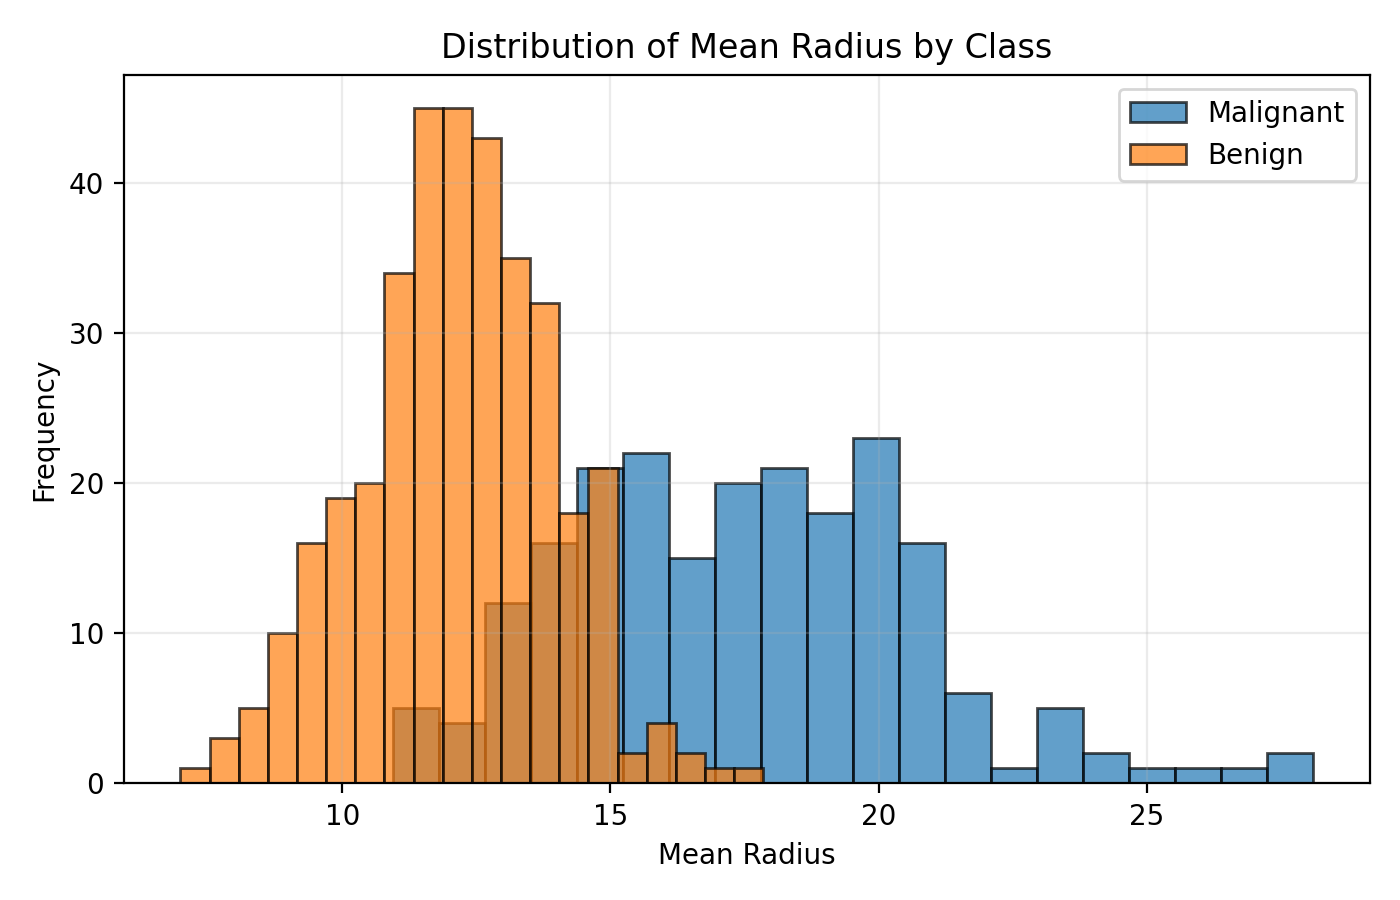
\includegraphics[width=0.78\textwidth]{mean_radius_hist.png}
    \caption{Histogram of mean radius, colored by class. Malignant and benign cases show noticeable separation, which suggests that this feature contains useful discriminative information.}
    \label{fig:hist}
\end{figure}

\subsection{Standardization}
Feature standardization was applied using zero-mean, unit-variance scaling. Importantly, the scaler was fitted \textbf{only on the training set}, and the learned transformation was then applied to validation and test sets.

This is necessary to prevent \textbf{data leakage}. If the scaler were fitted using validation or test data, the model would indirectly gain information from unseen samples through the normalization statistics. That would produce an overly optimistic evaluation. Fitting on the training set only ensures a fair estimate of generalization performance.

\section{k-NN Classifier}
\subsection{Hyperparameter tuning}
The homework requires trying the values
\[
k \in \{1,3,5,7,9,15,21\}.
\]
Each k-NN model was trained on the standardized training set and evaluated on the standardized validation set. The resulting validation accuracies are shown in Table~\ref{tab:knnval} and Figure~\ref{fig:knnval}.

\begin{table}[H]
\centering
\caption{Validation accuracy for different k values}
\label{tab:knnval}
\begin{tabular}{cc}
\toprule
$k$ & Validation accuracy \\
\midrule
1 & 0.9176 \\
3 & 0.9294 \\
5 & 0.9294 \\
7 & 0.9294 \\
9 & 0.9529 \\
15 & 0.9529 \\
21 & 0.9529 \\
\bottomrule
\end{tabular}
\end{table}

\begin{figure}[H]
    \centering
    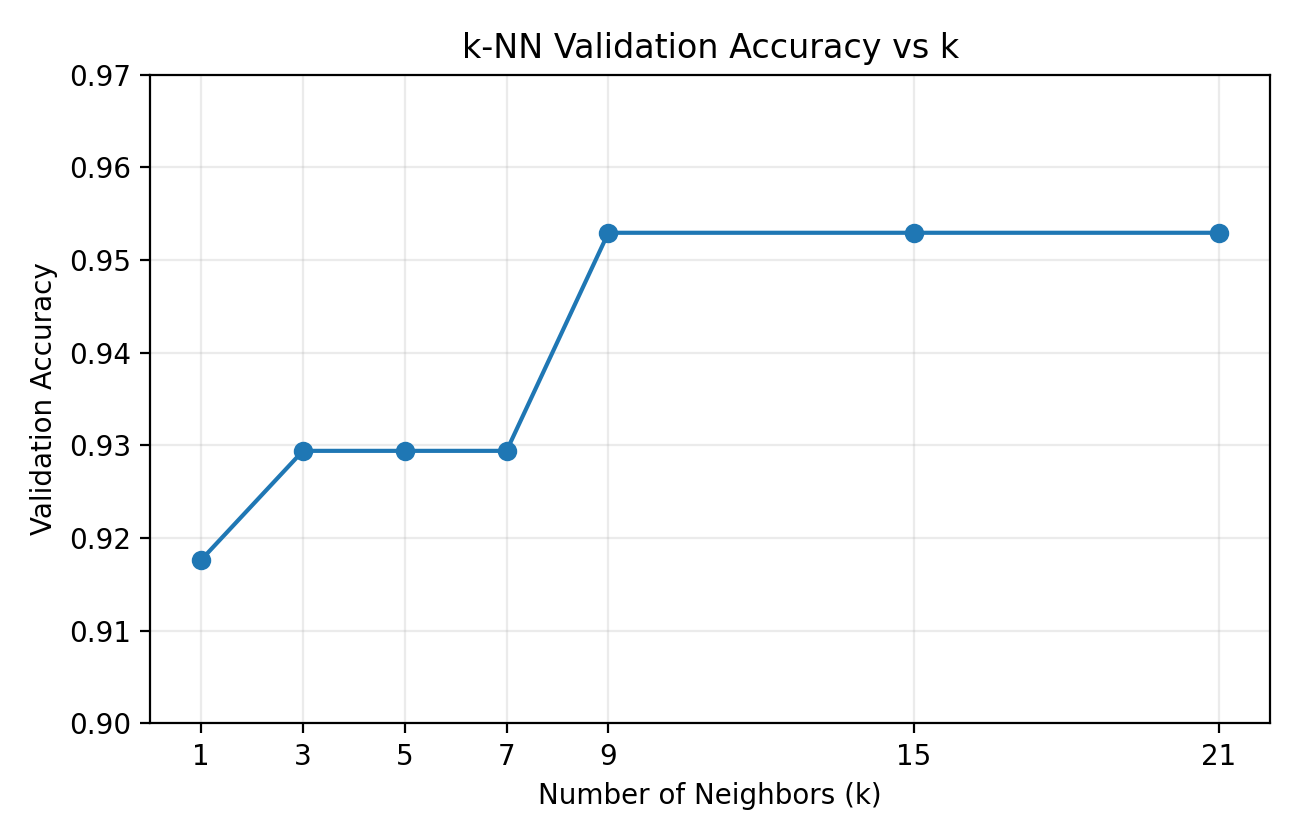
\includegraphics[width=0.72\textwidth]{knn_validation_accuracy.png}
    \caption{Validation accuracy of k-NN for different neighbor counts. In line with lecture intuition, larger values than $k=1$ smooth the decision rule and improve generalization, but excessively large values may eventually underfit.}
    \label{fig:knnval}
\end{figure}

The best validation accuracy is achieved by $k=9$, $k=15$, and $k=21$. To keep the model simple while preserving the best validation score, the smallest best value, \textbf{$k=9$}, was selected.

\subsection{Final k-NN model and test evaluation}
After selecting $k=9$, the training and validation sets were combined, the scaler was refit on this combined set, and the final k-NN model was evaluated on the test set.

\begin{table}[H]
\centering
\caption{Final k-NN test result}
\begin{tabular}{lc}
\toprule
Metric & Value \\
\midrule
Best $k$ & 9 \\
Test accuracy & 0.9884 \\
\bottomrule
\end{tabular}
\end{table}

\begin{figure}[H]
    \centering
    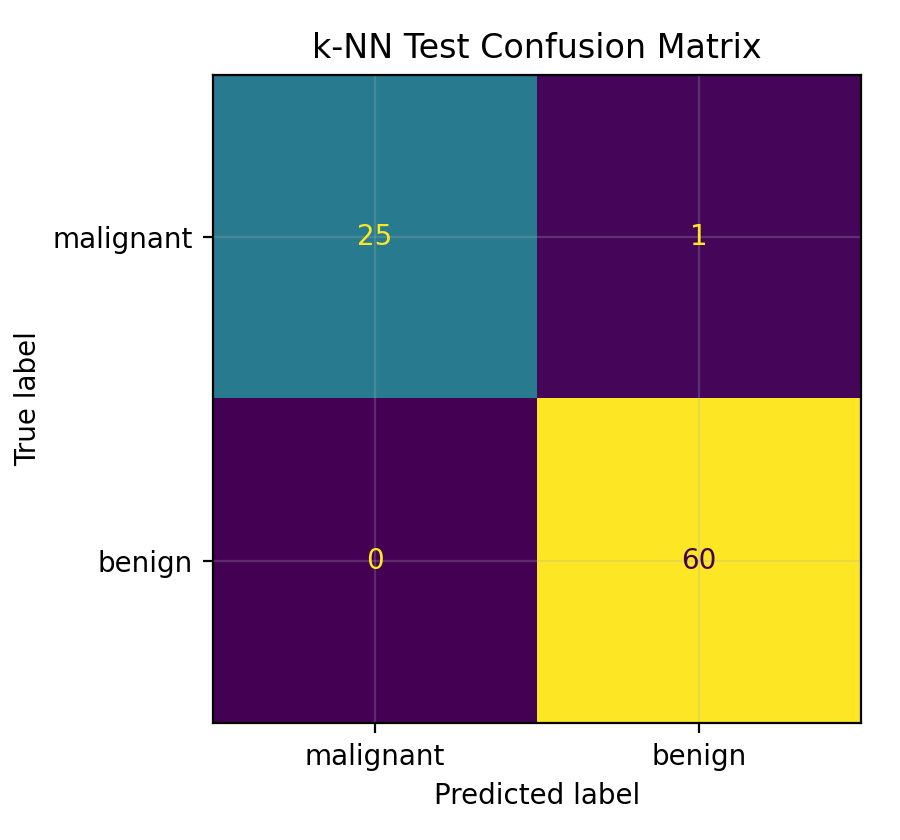
\includegraphics[width=0.48\textwidth]{knn_confusion_matrix.png}
    \caption{k-NN confusion matrix on the test set.}
\end{figure}

The confusion matrix is
\[
\begin{bmatrix}
25 & 1 \\
0 & 60
\end{bmatrix}
\]
with rows representing true labels and columns representing predicted labels.

This model makes only one mistake. It predicts one benign sample as malignant and does not miss any malignant sample in this split. Intuitively, the single error likely lies close to the class boundary in feature space, where its nearest neighbors are dominated by the opposite class.

\section{Decision Tree Classifier}
\subsection{Hyperparameter tuning}
The following hyperparameters were tuned using the validation set:
\begin{itemize}
    \item \texttt{max\_depth} $\in \{2,4,6,8,\texttt{None}\}$
    \item \texttt{min\_samples\_split} $\in \{2,5,10\}$
\end{itemize}

The validation accuracies for all configurations are visualized in Figure~\ref{fig:dtval}. The best validation accuracy was obtained by multiple settings, and the shallower configuration \textbf{max\_depth = 4} and \textbf{min\_samples\_split = 2} was chosen as the final validation winner because it reaches the top score with a simpler tree.

\begin{figure}[H]
    \centering
    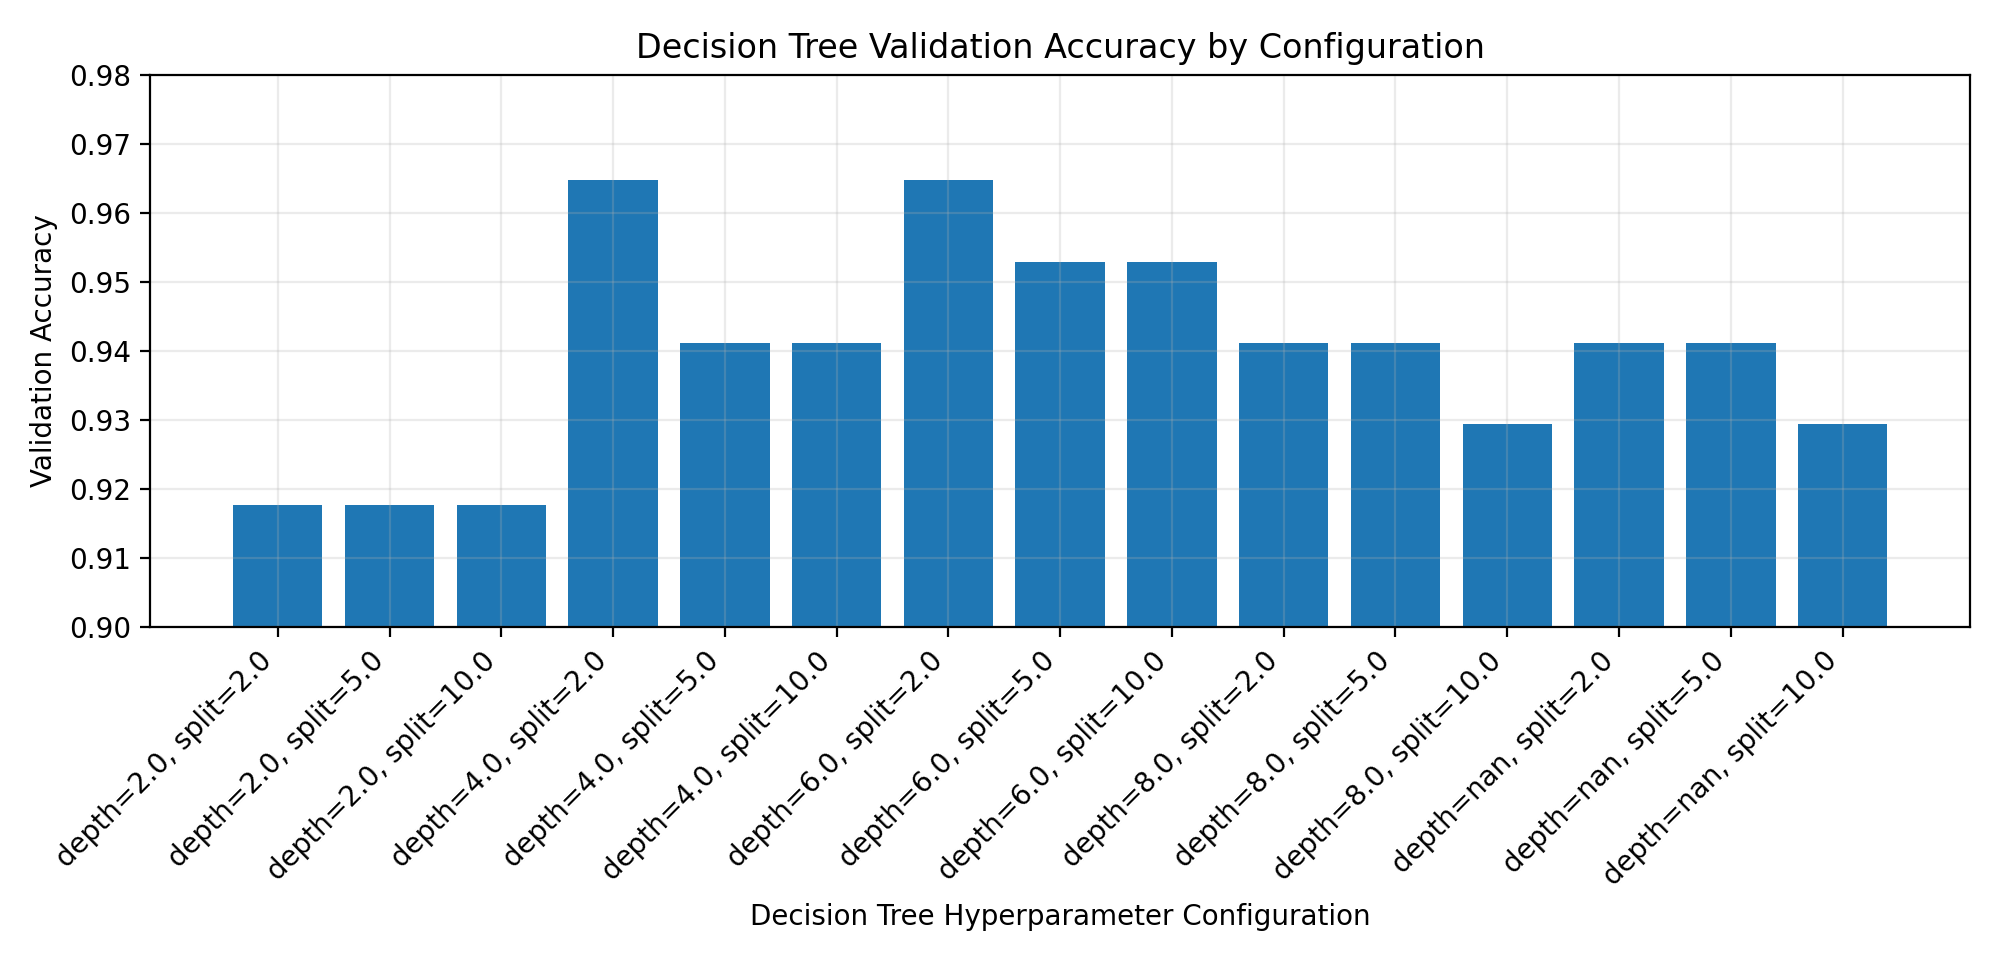
\includegraphics[width=0.95\textwidth]{dt_validation_accuracy.png}
    \caption{Validation accuracy for each Decision Tree hyperparameter configuration.}
    \label{fig:dtval}
\end{figure}

\subsection{Final Decision Tree and test evaluation}
The final Decision Tree was retrained on the combined training and validation sets, then evaluated on the test set.

\begin{table}[H]
\centering
\caption{Final Decision Tree test result}
\begin{tabular}{lc}
\toprule
Metric & Value \\
\midrule
Best max\_depth & 4 \\
Best min\_samples\_split & 2 \\
Test accuracy & 0.9535 \\
\bottomrule
\end{tabular}
\end{table}

\begin{figure}[H]
    \centering
    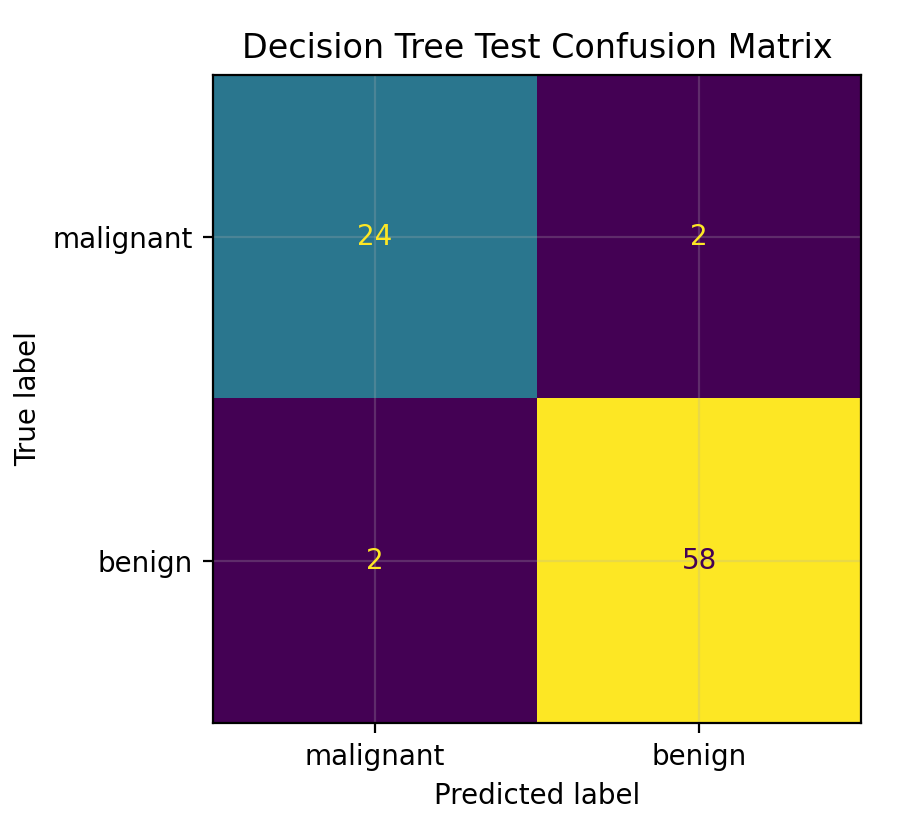
\includegraphics[width=0.48\textwidth]{dt_confusion_matrix.png}
    \caption{Decision Tree confusion matrix on the test set.}
\end{figure}

The confusion matrix is
\[
\begin{bmatrix}
24 & 2 \\
2 & 58
\end{bmatrix}
\]
which shows that the Decision Tree makes more errors than k-NN on this split, including both false positives and false negatives.

\subsection{Feature importance}
The feature importances of the best Decision Tree are shown in Figure~\ref{fig:featimp}. The most informative feature is \textbf{mean concave points}, which dominates the learned splits. Other useful features include worst concavity, worst area, worst texture, and worst perimeter.

\begin{figure}[H]
    \centering
    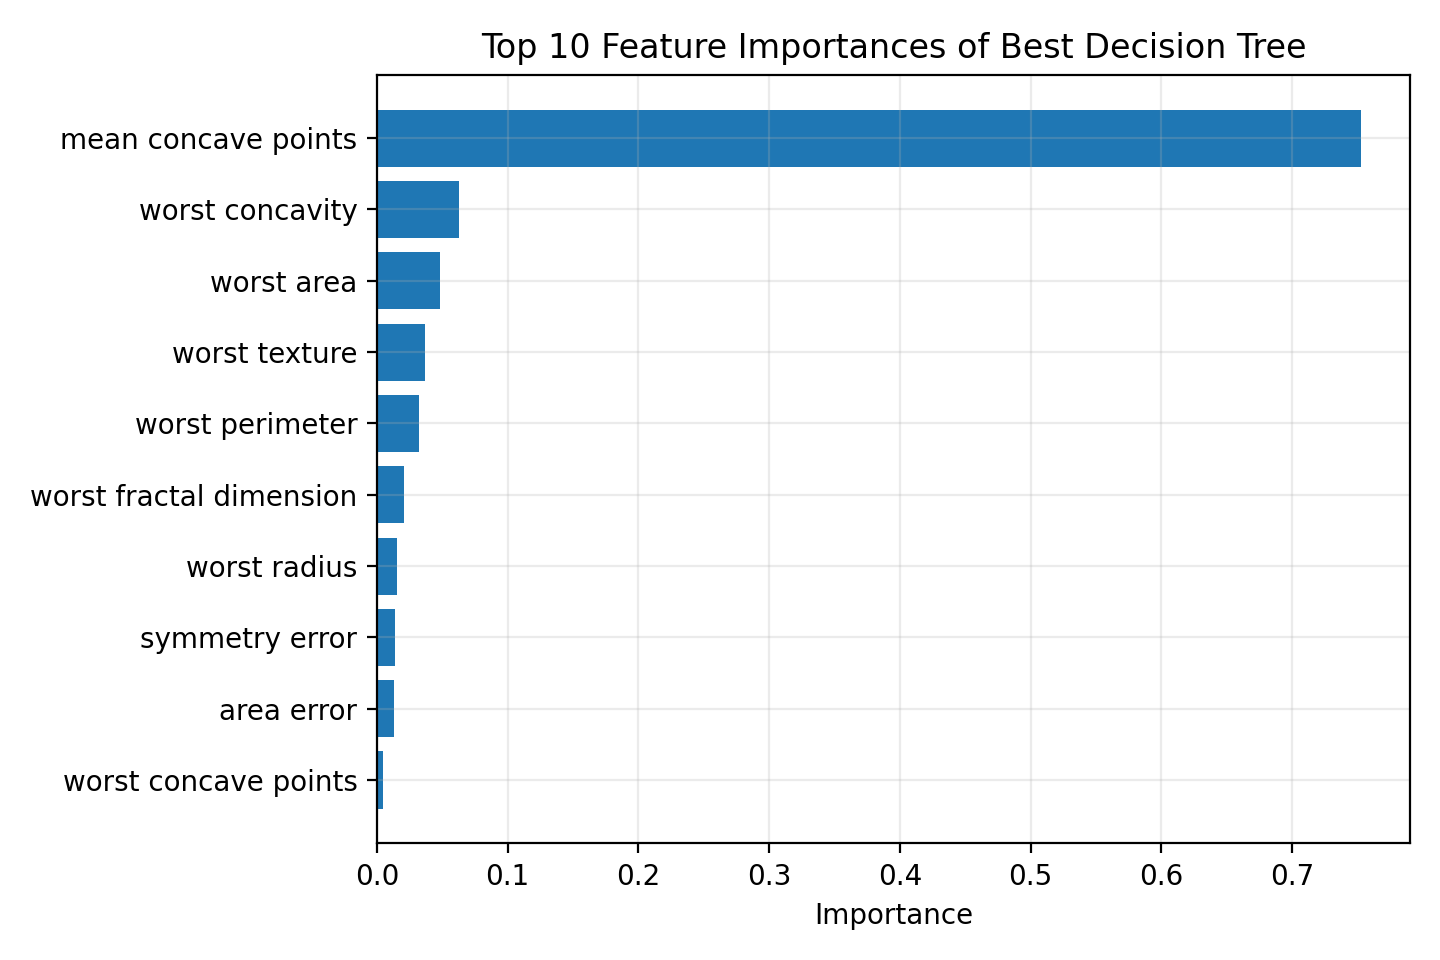
\includegraphics[width=0.82\textwidth]{dt_feature_importances.png}
    \caption{Top 10 feature importances of the best Decision Tree.}
    \label{fig:featimp}
\end{figure}

This result is consistent with the medical nature of the dataset because irregular boundary-related measurements help separate malignant and benign masses.

\section{Misclassification Analysis}
For \textbf{k-NN}, the model makes only one test-set error, and this error is a \textbf{false positive}. For \textbf{Decision Tree}, the model makes both \textbf{false positives} and \textbf{false negatives}. In a medical diagnosis context, the more critical mistake is a \textbf{false negative}, because predicting a malignant tumor as benign can delay further examination and treatment. Although false positives also have a cost, they are usually safer than missing an actual malignant case.

\section{Conclusion}
Both models achieve strong results on the Breast Cancer Wisconsin dataset, but \textbf{k-NN performs better in this homework}. Its test accuracy is \textbf{0.9884}, compared with \textbf{0.9535} for the Decision Tree, and its confusion matrix shows fewer mistakes. The Decision Tree remains valuable because it is more interpretable and provides feature importance information, but for this particular split and tuning setup, k-NN generalizes better.

\vfill
{\footnotesize Note: the notebook link above is a placeholder and should be replaced with the actual shareable notebook link before submission.}

\end{document}
